\section{METODOLOGI}

\subsection{Desain Robot yang Digunakan}

\begin{figure} [ht] \centering
	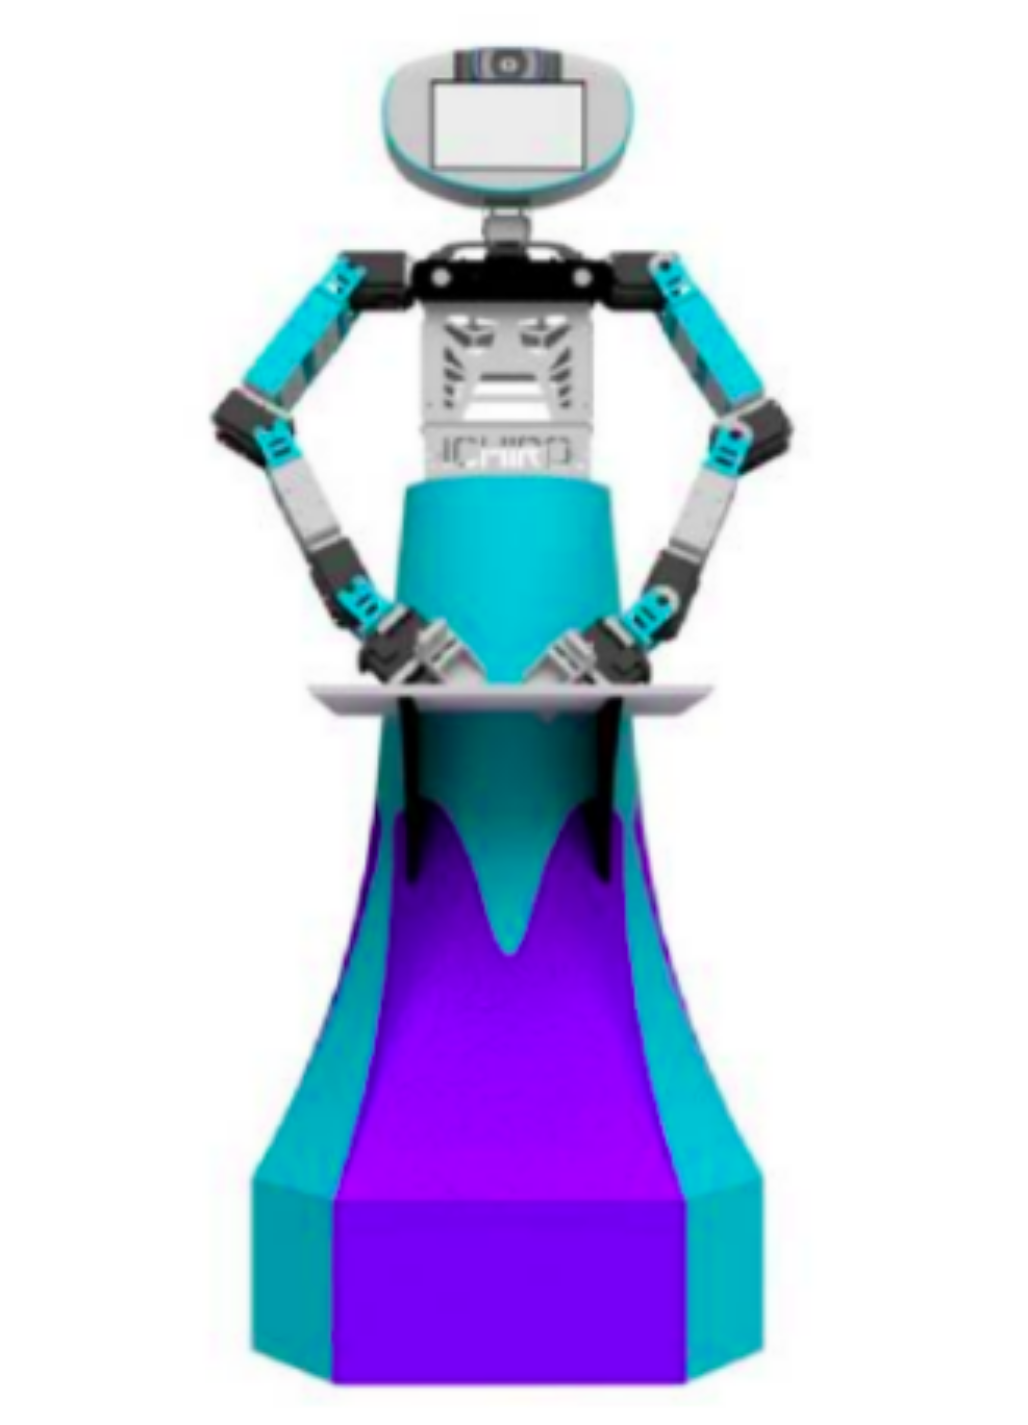
\includegraphics[scale=0.45]{gambar/robot-design.png}
	\caption{Desain Robot yang Digunakan}
	\label{fig:RobotDesign}
\end{figure}

Robot yang akan digunakan pada pada penelitian ini memiliki desain \emph{mobile humanoid robot} \citep{Mohamed2012}, yang merupakan gabungan antara robot mobile dan robot humanoid.
Seperti yang terlihat pada gambar \ref{fig:RobotDesign}, bagian bawah robot menyerupai robot mobile dengan \emph{differential wheels} yang memungkinkan pergerakan ke segala arah secara dua dimensi, sedangkan bagian atas robot menyerupai robot humanoid yang terdiri atas badan, kepala, dan lengan.
Dengan desain mobile humanoid robot ini, diharapkan pengguna bisa merasakan interaksi sosial yang lebih baik dengan robot karena memiliki bentuk mendekati manusia \citep{Rossi2018} sambil mempermudah navigasi dari robot ke berbagai tempat.

Robot ini dilengkapi dengan beberapa sensor seperti IMU (\emph{inertial measurement unit}) untuk mengetahui orientasi dari robot dan sensor kamera di kepala untuk mendeteksi objek menggunakan visi komputer.
Selain itu robot ini juga dilengkapi dengan dua lengan seperti robot manipulator yang bisa diatur pada berbagai posisi dan orientasi \citep{Iqbal2012}.
Dengan adanya sensor dan lengan ini diharapkan robot mampu melakukan tindakan assistive secara sosial sesuai dengan data yang didapatkan dari sensor yang ada.

\subsection{Pengembangan Sistem Robot}

Sistem robot dikembangkan menggunakan \emph{ROS 2}.

\subsection{Pembuatan Lingkungan Simulasi}

Lingkungan simulasi dibuat menggunakan \emph{Gazebo}.

\subsection{Pengujian Sistem Robot terhadap Lingkungan Simulasi}

Pengujian sistem robot akan dilakukan untuk setiap fungsionalitas yang dimiliki robot.
